\subsection{Product Perspective}
\subsubsection{Class Diagram}
The class diagram represented in Figure~\ref{fig:uml} represents the domain of the system. \\
The main elements in the class diagram are:
\begin{itemize}
    \item \textbf{User}: identifies two types of users who can access the application.\\
    \textsl{Farmer} and \textsl{Policy Maker} are the two categories of users that are present in the system. \\
    The distinction has to be applied in order to have different permissions.\\
    Users have a password used for the autentication and an email, in the case of a farmer, or an alphanumeric code, in case of a policy maker.
    \item \textbf{Farm}: stores all the information related to a Farm.\\ 
    It can be owned only by a farmer, and is located in a specific position visible by the map. \\
    It contains also the data about the production inserted by the farmer himself, that could be not present yet.
    (if a farmer has not started yet or has not inserted these information).\\
    Each farm is provided of sensors of two kind: one that collect data about the amount of water used by the farmer in his farm and humidity every day.\\
    \item \textbf{Notification}: this class represents content sent between users (in order to communicate something) or something submitted in the sistem that is stored in the database.
        \begin{enumerate}
            \item \textsl{Help}: it stores the single farmer that writes it, 
            the type of production he selects and a body where the farmer explains in details the problem.\\
            When this notification is sent to a policy maker, the system registers in it the actual date and time.
            \item \textsl{Advice}: the structure of it is the same as the Help class but it is not sent to anyone,
             it is immediatly stored in the database.
            \item \textsl{Evaluation}: this class represents the evaluation on exacly one farm by a single policy maker.\\ Each policy maker can evaluate one or more 
            farms more than once since this event happens once a month.\\ Despite it, an evaluation is related only to one farm and the result can be positive (1) or negative (0).\\ The evaluation is sent by the policy maker to the farm owner.
            \item \textsl{Solution}: this class is like the Help one, in fact is the reply of a policy maker to a help request within the body the solution found by the sender.
        \end{enumerate}
    
    \item \textbf{Map}: this object contains a list of all the farms located in Telegana and registered in the application.\\It stores all the information about the farms in order to provide them to the users.
    \item \textbf{Weather Info}: this class is a representation of the meteorological information of the country, provided by an external application.\\These information are specific for each position in which a farm is located.
    
    \item \textbf{Forum}: here are stored all the messages sent by the farmers on the forum page.\\ It allows the system to make the messages always visible to all the farmers.\\ In addition to that the messages are also ordered by date and time in which they were sent.
    
\end{itemize}
\begin{figure}[H]
    \begin{center}
    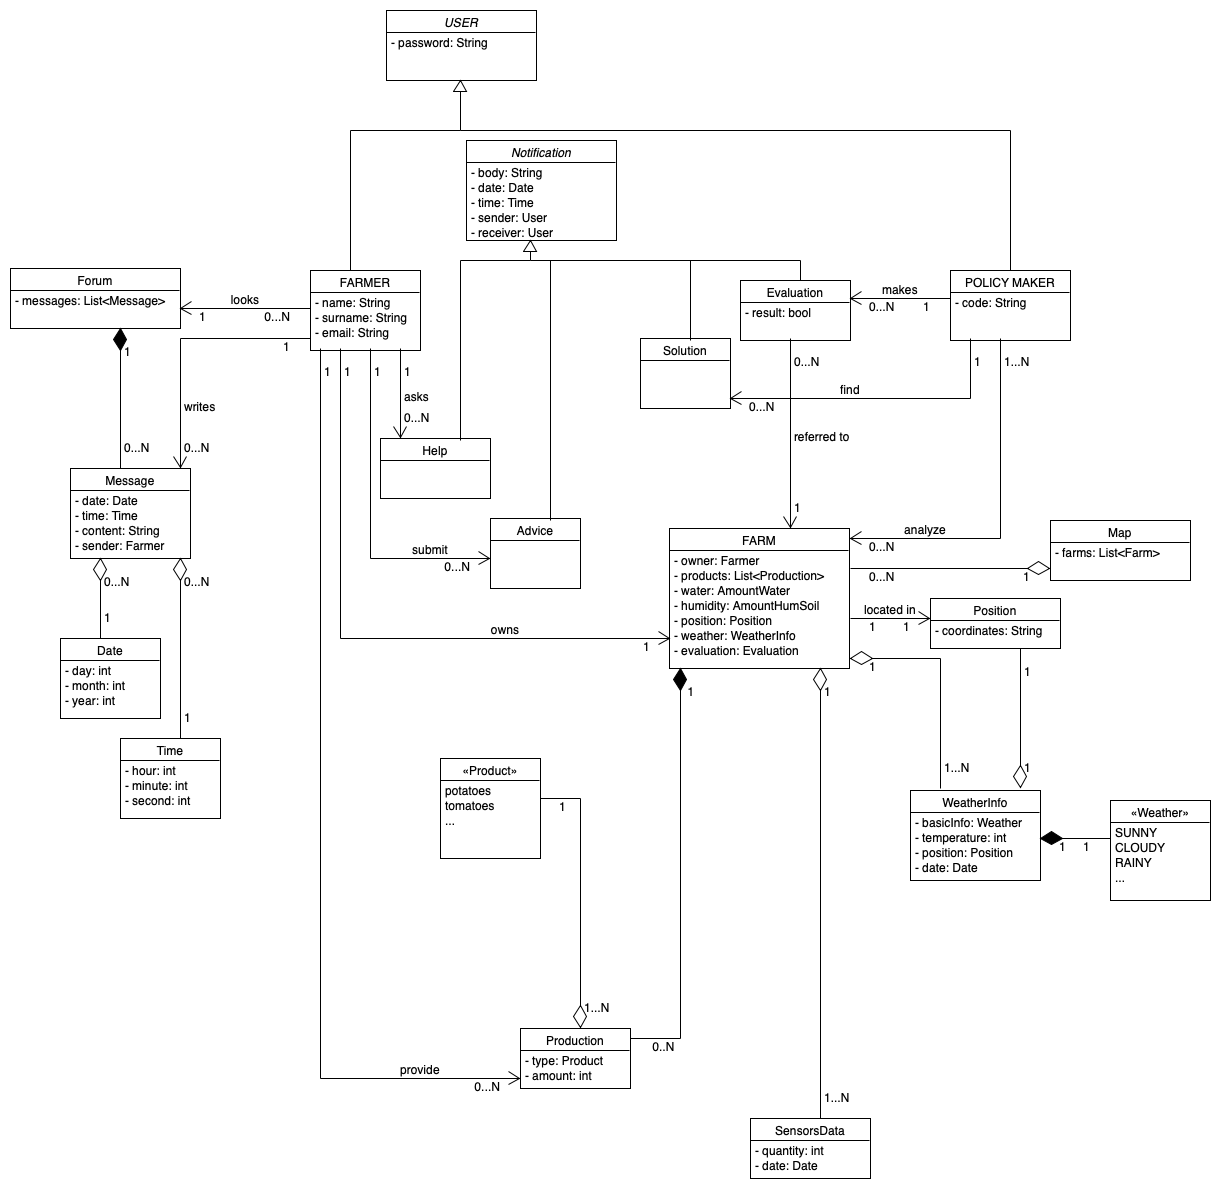
\includegraphics[width=1\textwidth]{images/UML.png}
    \caption{UML diagram.}
    \label{fig:uml}
    \end{center}
\end{figure}
\newpage
\subsubsection{State Diagrams}
The following state diagrams describe the behavior of the main objects of the system's domain previously described(Figure~\ref{fig:uml}). 
They consider all the potentional states that the element examined can have 
while a certain event takes place.

\begin{enumerate}
    \item \textbf{Update of the Farmer Page}
        The state diagram represented in figure~\ref{fig:state1} represents 
        the events that might occur whenever the farmer page is updated.
        The three main circumstances when the page is updated are:
        \begin {itemize}
        \item Farmer inserts new production data
        \item There is new data available on weather forecast
        \item Sensors collect new data
        \end{itemize}
        The page is so updated after one of this events occurs.

    \begin{figure}[H]
        \begin{center}
        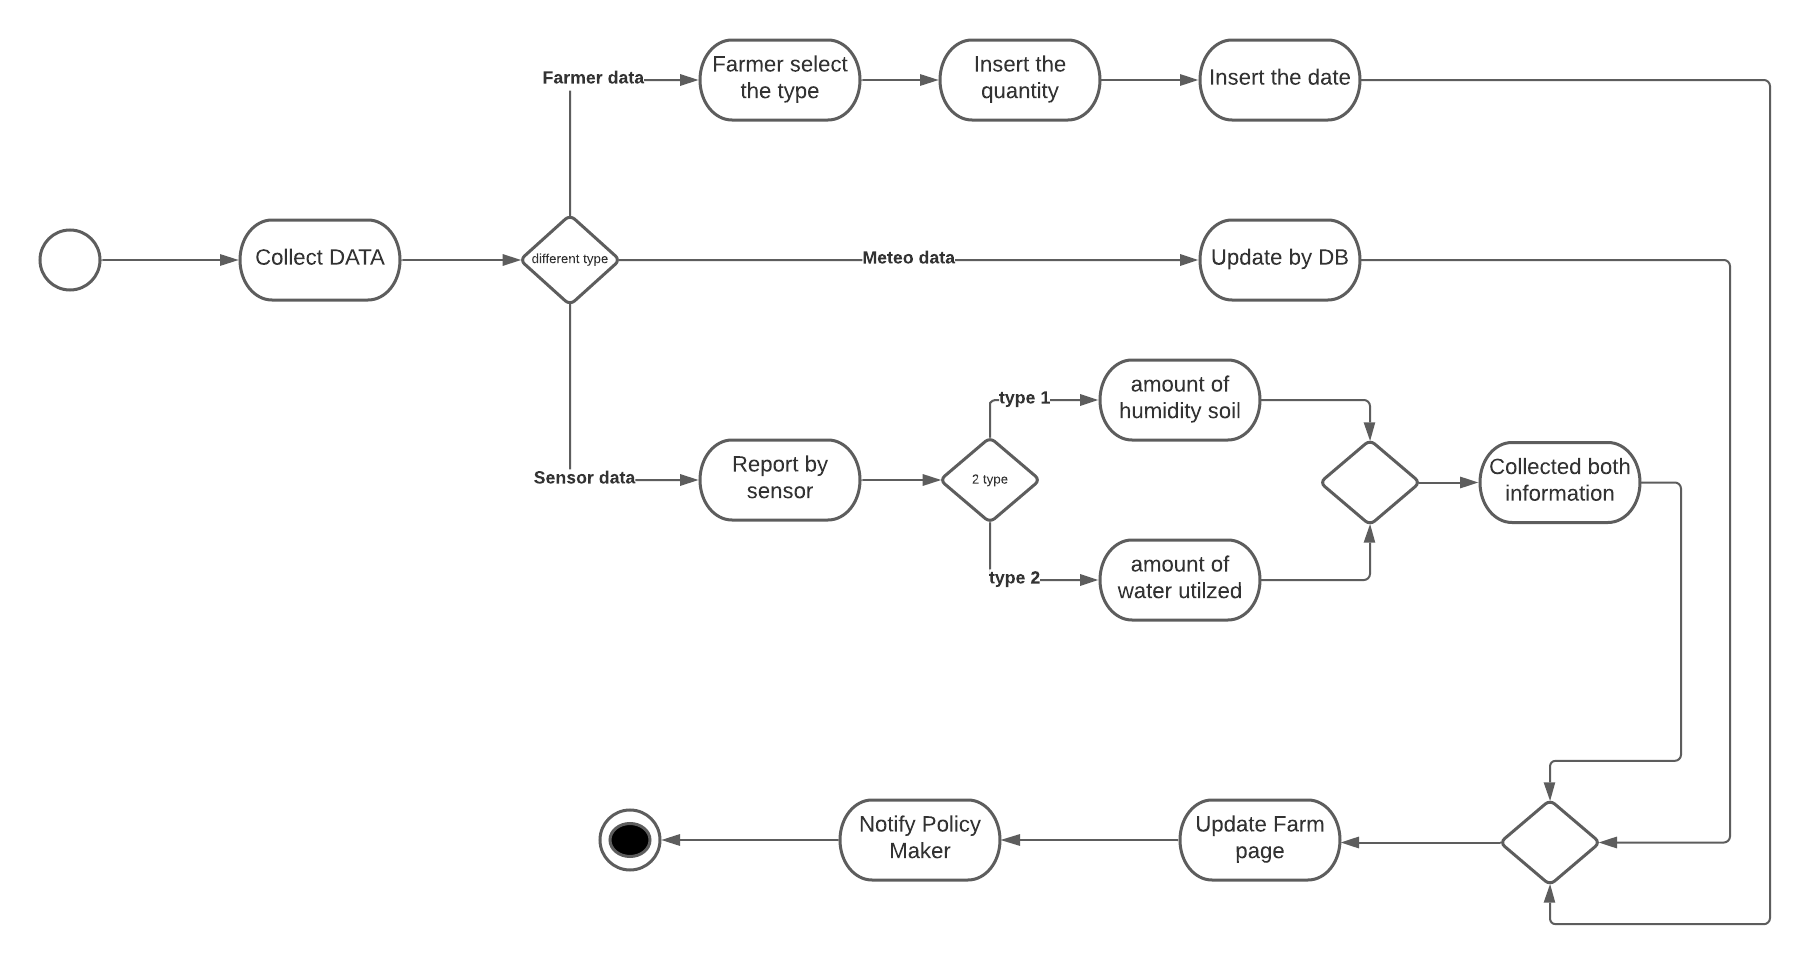
\includegraphics[width=1\textwidth]{images/State chart 1.png}
        \caption{Update Farmer page.}
        \label{fig:state1}
        \end{center}
    \end{figure}

    \item \textbf{Analysis of different farmers}
    The state diagram in figure \ref{fig:state2} represents the analysis that is performed 
    by the policy makers once a month.
    As a matter of fact the policy maker starts the analysis after selecting the farm, he visualizes then the farmer's farm page and analyzes the information 
    that is present in it. After the anlaysis the map is updated and the system sends a notification, that is then different if the 
    farmer’s performance is either good or bad.

    \begin{figure}[H]
        \begin{center}
        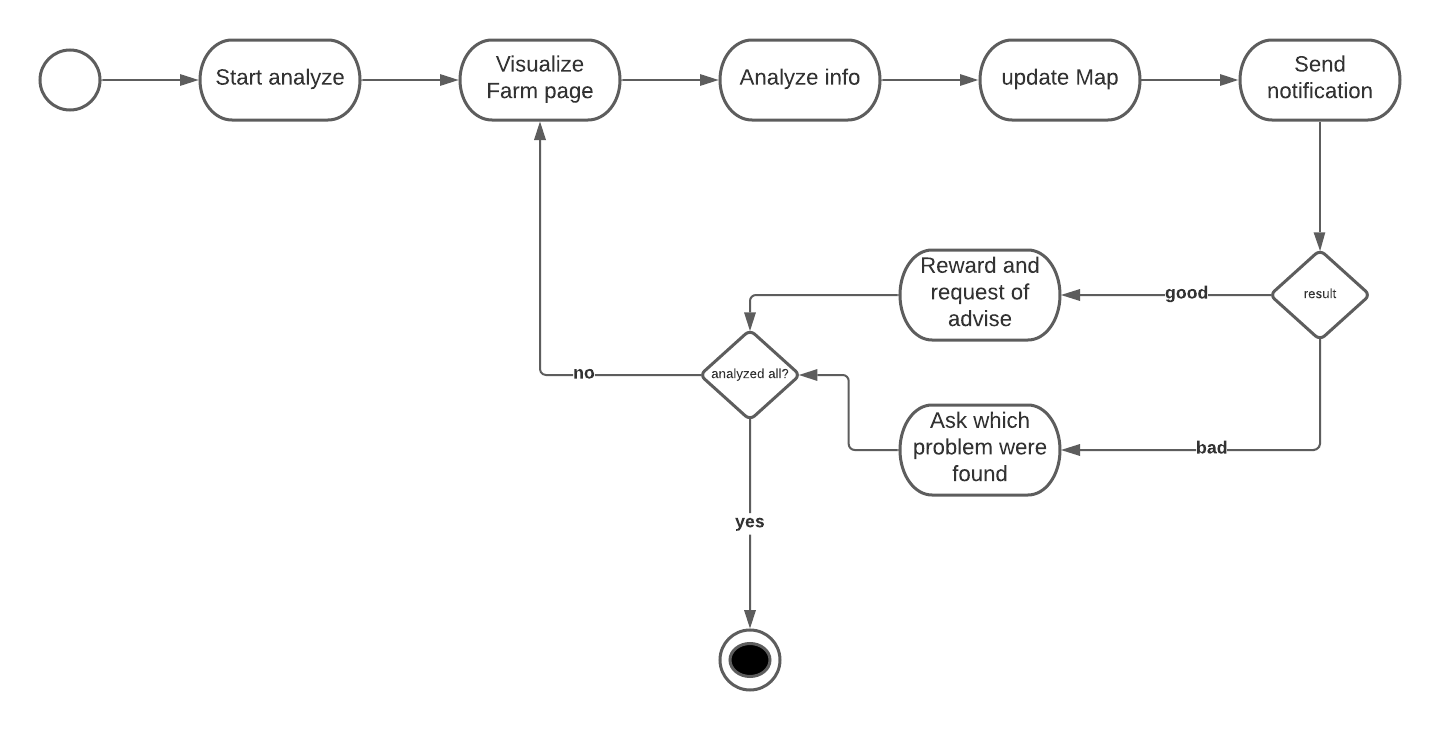
\includegraphics[width=1\textwidth]{images/State chart 2.png}
        \caption{Analysis of farmers.}
        \label{fig:state2}
        \end{center}
    \end{figure}

    \item \textbf{Request of help from a farmer}
    \item The diagram represented in Figure \ref{fig:state3} shows the events that takes place 
    when a farmer sends a request of help. It can happen either by writing a message in the forum 
    or by sending a request through a form in the homepage.
    \begin{figure}[H]
        \begin{center}
        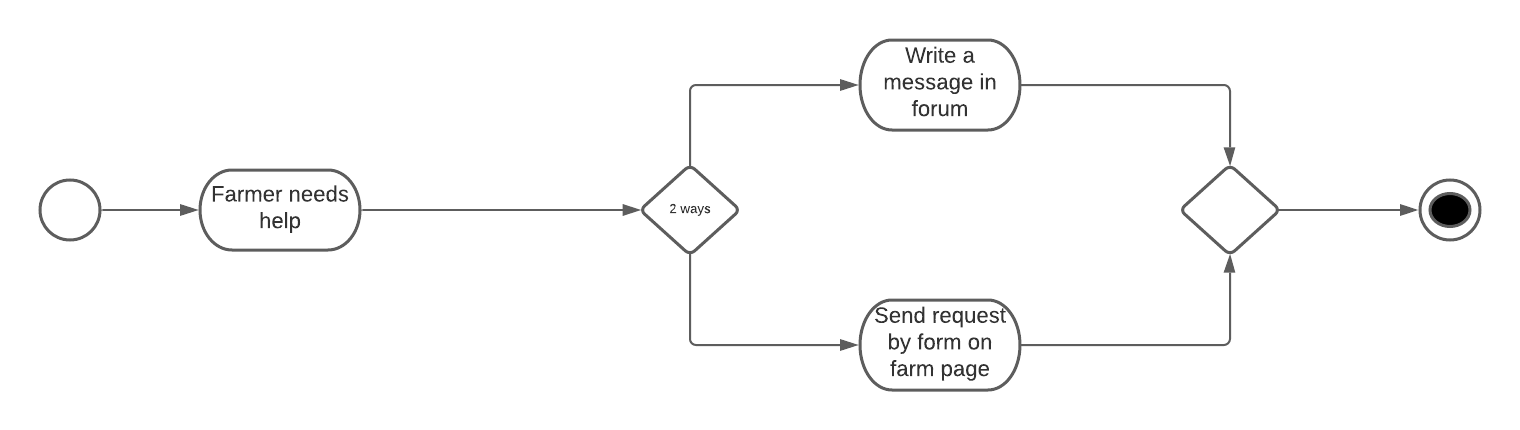
\includegraphics[width=1\textwidth]{images/State chart 3.png}
        \caption{Request of help.}
        \label{fig:state3}
        \end{center}
    \end{figure}
\end{enumerate}
\newpage
\subsection{Product Functions}\label{subsection:2.2}
This section provides a summary of the main features and 
functions offered by the software regarding
the goals already described in section~\ref{section:1.1.1}.

In the following description it is important to highlight that both
the policy makers and the farmers must be logged in.

\subsubsection{Farmers insert data} 
This functionality is accessible to all farmers.\\
The application provides a form in which a farmer can easily insert data of his production.
The form is easy to fill in, in order to complete it the farmer needs to specify:
\begin{itemize}
    \item the \textbf{type of product}
    \item the \textbf{amount} producted of the selected type
    \item the \textbf{date} relative to the date of the production
\end{itemize}
If the farmer needs to add more than one type of product, 
he can fill in the form multiple times.\\
After completing the form the user is redirected to his updated farm's page and the policy makers 
can see the updated data.\\
This functionality can be done more than once a day since the farmer can select the date, 
so it is possible for him to insert data of past days too.



\subsubsection{Farmers visualize data}
This functionality lets the farmer visualize all the data 
acquired from the system. The farmer can visualize all data on his homepage.\\
The application shows:
\begin{itemize}
    \item meteorological  short-term and long-term forecast
    \item amount of water used by the farmer
    \item humidity of soil 
    \item list of all his past productions
\end{itemize}

\noindent This functionality is always up to date, and does not need 
any input from the farmer.
It is used by the farmer only to have a general view of 
his farm.



\subsubsection{Identify how farmers are performing}
The main feature of the policy makers is to evaluate the work of each farmer. 
In order to do that, they periodically analyze each farm page: 
the system allows them to visualize all the data in those pages 
(but not to modify it).\\
The analysis takes place once a month.\\
With this analysis they classify the workers in two different way:
\begin{itemize}
    \item GOOD farmer : those how have been able to produce a significant amount of product with low resources, despite bad weather in that period.
    \item BAD farmer : those who did not produce much.
\end{itemize}
Policy makers inform each farmer the result they have achieved with a notification: 
\begin{itemize}
    \item GOOD farmers receive a special 
    incentive, and also a request to submit 
    from their personal web page some advice that could be useful to the others. 
    \item To BAD farmers is asked to submit an explicit request of help specifying the problems they had.
\end{itemize}
The system has a specific web page that allows all 
the users to look at a map of the area in which there are 
specified all the farms. It is also shown if the farm's owner has performed 
a good job in that period.
At the end of each analysis the policy makers 
update the map (they are the only ones that are able to modify it).


\subsubsection{Interaction between farmers}
This functionality permits the farmers to communicate with each other. 
The application has a specific web page were the farmers can send messages 
whenever they want.\\
If a farmer has an issue, before submitting a formal request of help to 
the policy makers 
by their farm's page, he can ask informally an advice by sending a message 
in the forum.
It is not necessary to be a good farmer in order to answer someone elses 
message.\\ All the messages are visible to everyone and 24h. 
Since it is an online application an internet connection is required 
to read or write on this page.

%---------------------------------------------------------------------------%
\subsection{User Characteristics}
Dream has two different customers that need to be 
distinguished in order to provide the various 
features specified in subsection ~\ref{subsection:2.2}.

\subsubsection{Farmer}
\begin{itemize}
    \renewcommand\labelitemi{--}
    \item Can register on Dream in order to be recognized as farmer
    \item Must log in on the website to use the services offered
    \item Can discuss with other farmers
    \item Is able to insert data about their daily production
    \item Can ask for help to other farmers or to policy makers
    \item Can retrieve data regarding weather forecast, water irrigation system or humidity of soil
    \item Can give and ask for advice on several products
    \item Can check whether their performance is identified as good or bad
\end{itemize}

\subsubsection{Policy Maker}

\begin{itemize}
    \renewcommand\labelitemi{--}
    \item Already has the credential to access to the system
    \item Must login to Dream to benefit of its services
    \item Can look all farms' pages
    \item Can update the map
    \item Can send suggestions to whom explicitly notices a problem
    \item Can send notifications to the farmers
    \item Decides the value of the incentive for the good farmers
    \item Evaluates the performance of the farmers
\end{itemize}


\subsection{Domain Assumptions, Dependencies and Constraints}
This subsection focuses on what it is assumed in order for our system to offer the services as expected.
Moreover it focuses on the limitations that the system could face.

\subsubsection{Domain Assumptions}
\textbf{DA1} In order to access the system users need to have Internet connection.\\
\textbf{DA2} Farmers always insert correct data on their production activity.\\
\textbf{DA3} Data from sensors is always correct.\\
\textbf{DA4} Date and Time on the system are always correct.\\
\textbf{DA5} The position of the Farm is always correct.\\
\textbf{DA6} Internet connection works always without errors.\\
\textbf{DA7} Meteorological data is accurate.\\
\textbf{DA8} Every farm has a different position.\\
\textbf{DA9} Each farm belongs to exacly one farmer.\\
\textbf{DA10} Discussion on the forum are related only to the farm activity.\\
\textbf{DA11} Formal request of help must be related to a farmer's own production.\\
\textbf{DA12} Advice on a product must be given by a farmer that produces the same type.\\
\textbf{DA13} Performances of farmers are always identified correctly.\\
\textbf{DA14} Farmers can insert data more than once a day.\\
\textbf{DA15} The email and farm's name must be unique.\\
\textbf{DA16} Policy Makers have a given code and password to access the system.\\
\textbf{DA17} All farmers that sign up own a real farm in Telengana.\\
\textbf{DA18} The special incentive that the farmers receive for their good work, is used on stuff related to their farm activity.\\

